%%%%%%%%%%%%%%%%%%%%%%%%%%%%%%%%%%%%%%%%%
%
% (c) 2021 by Jennifer Laaser
%
% This work is licensed under the Creative Commons Attribution-NonCommercial-ShareAlike 4.0 International License. To view a copy of this license, visit http://creativecommons.org/licenses/by-nc-sa/4.0/ or send a letter to Creative Commons, PO Box 1866, Mountain View, CA 94042, USA.
%
% The current source for these materials is accessible on Github: https://github.com/jlaaser/pogil-polymers
%
%%%%%%%%%%%%%%%%%%%%%%%%%%%%%%%%%%%%%%%%%

\renewcommand{\figpath}{content/polymphys/chain-confs/chain-models/figs}
\renewcommand{\labelbase}{chain-models}

\begin{activity}{Models for Ideal Polymer Chains}

\begin{instructornotes}

	This activity introduces students to the concept of conformations of polymer chains.
	
	After completing this activity, students will be able to:
			\begin{enumerate}
				\item Describe the properties of random walks relevant for understanding polymer chains
				\item Identify simple models for polymer chains and describe their similarities and differences
				\item Express the properties of polymer chains in terms of their characteristic ratio and/or Kuhn length
				\item Calculate the radius of gyration for polymer chains, and understand how this quantity scales with changes in a polymer's molecular weight
			\end{enumerate}
	
			
	\subsection*{Activity summary:}
	\begin{itemize}
		\item \textbf{Activity type:} Learning Cycle
		\item \textbf{Content goals:} Basics of Chain Conformations
		\item \textbf{Process goals:} %https://pogil.org/uploads/attachments/cj54b5yts006cklx4hh758htf-process-skills-official-pogil-list-2015-original.pdf
			\begin{itemize}
				\item Interpreting mathematical equations in terms of physical behavior
				\item Oral and written communication of reasoning
			\end{itemize}
		\item \textbf{Duration:} approx. 45 minutes, including time for class discussion
		\item \textbf{Instructor preparation required:} 
			\begin{itemize}
				\item None beyond knowledge of relevant content
			\end{itemize}
		\item \textbf{Related textbook chapters:}
			\begin{itemize}
				\item \emph{Polymer Chemistry} (Hiemenz \& Lodge): Sections 6.1-6.3
				\item \emph{Polymer Physics} (Rubinstein \& Colby): Chapter 2
			\end{itemize}
	\end{itemize}
	
	\subsection*{Other notes:}
	
		\begin{itemize}
		\item If you choose to use Exercise \ref{\labelbase:exc:statseg}, please note that it most closely follows the treatment in section 2.2 of \emph{Polymer Physics} by Rubinstein \& Colby (in which $N$ in the equivalent freely jointed chain is \emph{not} equal to the actual degree of polymerization of the polymer, and $b$ is the Kuhn length) rather than that in Hiemenz \& Lodge (in which $N$ in the equivalent freely-jointed chain \emph{is} equal to the actual degree of polymerization of the polymer, and the statistical segment length $b$ is not the same as the Kuhn length).  The definitions in this exercise most closely follow
		\end{itemize}

\end{instructornotes}

	%\textbf{Focus question:} Put a central question for the students to consider through this exercise here.

\begin{model}[Random Walks]
\label{\labelbase:mdl:randomwalks}

	The simplest model for a polymer chain is a \emph{freely-jointed chain} consisting of $n$ links of length $l$ that can each point in any direction, regardless of the direction of the previous link.
	
	To understand the properties of a freely-jointed chain, we will first consider a simple one-dimensional model in which each link can point either to the right or the left with equal probability.

\end{model}


\begin{ctqs}

	\question Suppose the beginning of the chain is at $x=0$, and each link has length $l=1$.
	
		\begin{enumerate}
			\item What is the probability that, after the first link, you are at position $x=1$?
			
				\emph{(Hint: remember that each link has an equal probability of pointing to the right or to the left!)}
				
				\begin{solution}[0.5in]
				
					1/2
					
				\end{solution}
				
			\item Similarly, what is the probability that, after the first link, you are at position $x=-1$?
				
				\begin{solution}[0.5in]
				
					1/2				
				
				\end{solution}
			
		\end{enumerate}
		
	\question Building off your answers to the previous question, what are the probabilities that after the \emph{second} link you will be at...
	
		\begin{enumerate}
			
			\item ... position $x=2$?
			
				\emph{(Hint: remember that to get a total probability, we \emph{multiply} the probabilities of each step leading to the final outcome.)}
				
				\begin{solution}[1in]
				
					$\frac{1}{2}\frac{1}{2} = \frac{1}{4}$
				
				\end{solution}
				
			\item ... position $x=-2$?
				
				\begin{solution}[1in]
				
					$\frac{1}{2}\frac{1}{2} = \frac{1}{4}$
					
				\end{solution}
			
			\clearpage
			\item ... position $x=0$?
				\emph{(Hint: how many ways could you get to this final position?)}
				
				\begin{solution}[1in]
				
					There are two possible paths: $0\to 1\to 0$ and $0 \to -1 \to 0$.  Each occurs with probability $\frac{1}{2}\frac{1}{2} = \frac{1}{4}$ for a total probability of $2\cdot\frac{1}{4} = \frac{1}{2}$.
				
				\end{solution}
			
		\end{enumerate}
		
	\question Plot the probabilities you calculated in the previous question on the axes below:
	
		\begin{solution}[2.25in]
		\studentdisplay{
			\centerline{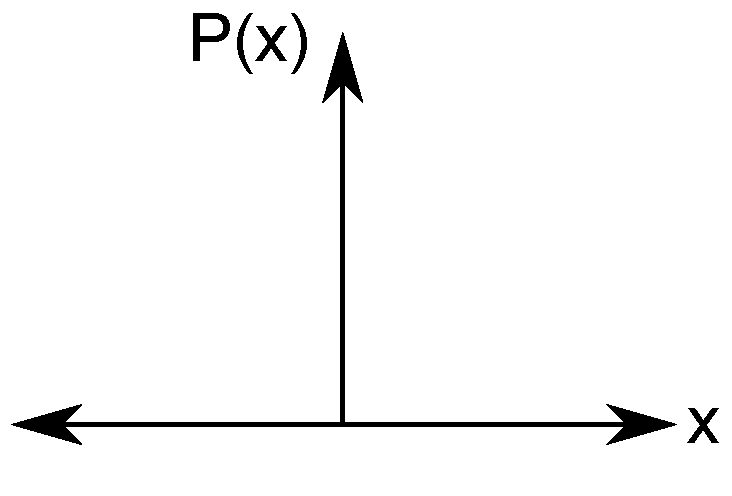
\includegraphics[width=0.45\textwidth]{\figpath/Model1_probability_axes}}
		}\instructordisplay{
			\centerline{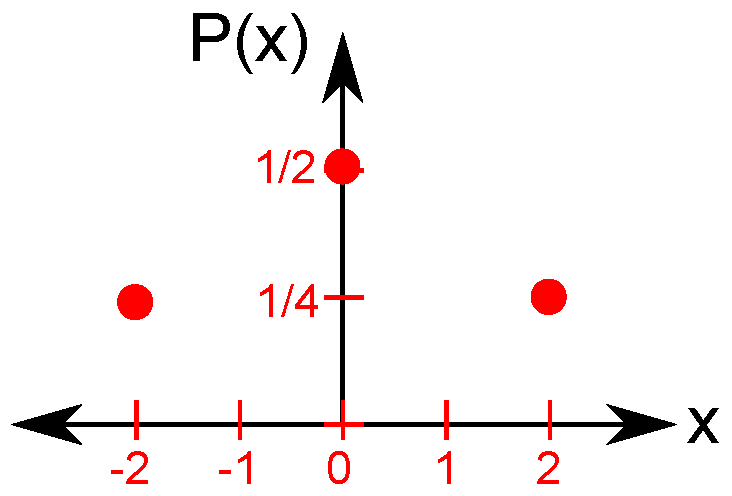
\includegraphics[width=0.45\textwidth]{\figpath/Model1_2steps}}
		}
		\end{solution}
	
	\question Predict what the probability distribution might look like after 100 links:
	
		\begin{solution}[2.25in]
		\studentdisplay{
			\centerline{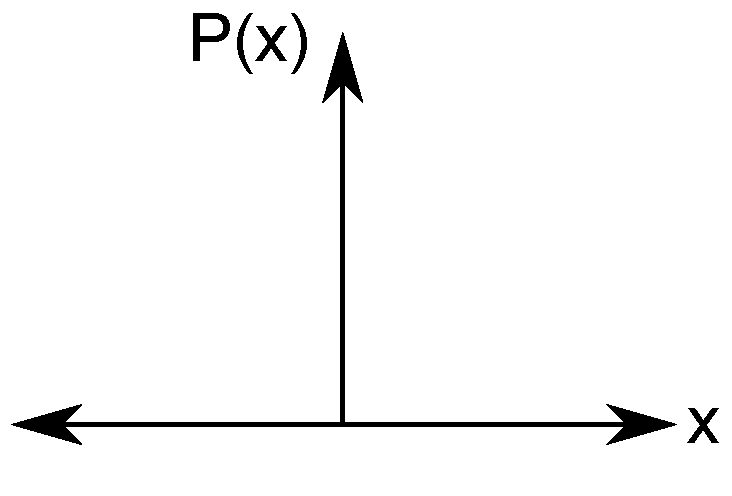
\includegraphics[width=0.45\textwidth]{\figpath/Model1_probability_axes}}
		}\instructordisplay{
			\centerline{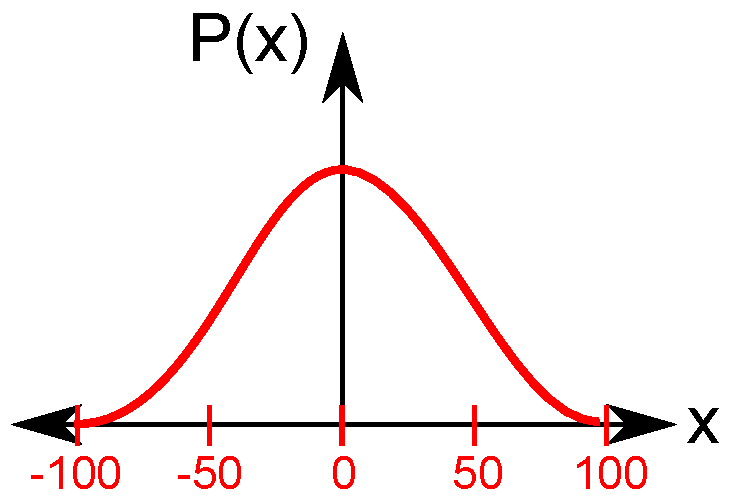
\includegraphics[width=0.45\textwidth]{\figpath/Model1_allsteps}}
		}
		\end{solution}
	
\end{ctqs}

\begin{infobox}
	
	The process you have investigated in the previous questions is called a \emph{random walk}.
	
	It is possible to show that after $n$ steps, the probability of being at position $x$ is approximately
	\begin{equation*}
		P(n,x) = \frac{1}{\sqrt{2\pi n}}e^{-x^2/2n}
	\end{equation*}
	
\end{infobox}

\begin{ctqs}

	\question As you know, in polymer science, we usually have to calculate \emph{average} properties over all of the possible conformations of the polymer chains.
	
		The average value of any function of $x$, $\langle f(x)\rangle$, can be calculated using
		\begin{equation*}
			\langle f(x) \rangle = \int_{-\infty}^\infty f(x) P(n,x)\,dx
		\end{equation*}
		
		\begin{enumerate}
			\item Evaluate the average final position, $\langle x \rangle$, for the 1D random walk described above.
			
				\emph{Hint: you will probably find one of the following integrals useful:}
				\begin{align*}
					\int_{-\infty}^\infty e^{-a x^2} = \sqrt{\frac{\pi}{a}} && \int_{-\infty}^\infty x e^{-a x^2} = 0 && \int_{-\infty}^\infty x^2 e^{-a x^2} = \frac{1}{2}\sqrt{\frac{\pi}{a^3}}
				\end{align*}
				
				\begin{solution}[1.5in]
					\begin{align*}
						\langle x \rangle &= \int_{-\infty}^\infty x \frac{1}{\sqrt{2\pi n}}e^{-x^2/2n}\, dx\\
						&= \frac{1}{\sqrt{2\pi n}} \int_{-\infty}^\infty x e^{-x^2/2n}\, dx\\
						&= \frac{1}{\sqrt{2\pi n}} \cdot 0\\
						&= 0
					\end{align*}
				\end{solution}
				
			\item Why is $\langle x \rangle$ not a particularly useful way to describe the properties of a polymer chain?  Explain your group's reasoning in 1-2 complete sentences.
				
				\begin{solution}[1.5in]
					No, $\langle x \rangle$ (which is the average position of the end of the chain) is not a particularly useful way to describe the chain's properties because it always comes to zero and does not depend on the number of steps in the chain.  
					
					Qualitatively, this is because there is an equal probability of finding the end of the chain to the right and to the left, so the average always just ends up right in the middle no matter how ``large'' the chain actually is.
				\end{solution}
			
		\end{enumerate}
		
	\question Suppose you instead wanted to calculate the mean square end-to-end distance of your chain, $\langle x^2\rangle$.
	
		\begin{enumerate}
			\item Write down an appropriate integral for this quantity and evaluate it as above.
				
				\begin{solution}[1.5in]
					\begin{align*}
						\langle x^2 \rangle &= \int_{-\infty}^\infty x^2 \frac{1}{\sqrt{2\pi n}}e^{-x^2/2n}\, dx\\
						&= \frac{1}{\sqrt{2\pi n}} \int_{-\infty}^\infty x^2 e^{-x^2/2n}\, dx\\
						&= \frac{1}{\sqrt{2\pi n}} \frac{1}{2}\sqrt{\frac{\pi}{(1/2n)^3}}\\
						%&= \frac{1}{2}\sqrt{\frac{8\pi n^3}{2\pi n}} \\
						%&= \frac{1}{2}\sqrt{4n^2}
						&= n
					\end{align*}
				\end{solution}
			
			\item Is $\langle x^2 \rangle$ a more useful measure of the size of a polymer chain?  Explain your group's reasoning in 1-2 complete sentences.
				
				\begin{solution}[1.5in]
				
					Yes, $\langle x^2 \rangle$ is a more useful measure of the size of a polymer chain, because it does depend on $n$.
					
					Note: here we consider the mean-square end-to-end distance, but it is also worth noting for students that the \emph{root mean square} (r.m.s.) end-to-end distance is $\sqrt{n}$.
				
				\end{solution}
		\end{enumerate}
		

\end{ctqs}

\begin{model}[Models for Polymer Chains]
\label{\labelbase:mdl:chainmodels}

	As noted in Model \ref{\labelbase:mdl:randomwalks}, the simplest model for a polymer chain is one in which each bond can point in any direction, regardless of the direction of the previous bond, as illustrated below.
	
		\centerline{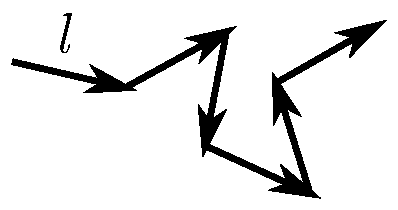
\includegraphics[width=0.2\textwidth]{\figpath/Model2_freelyjointed}}
	
	This model is called a \emph{freely-jointed} chain, and it is possible to show that the mean square end-to-end distance for a freely-jointed chain with $n$ bonds of length $l$ is given by
	\begin{equation*}
		\langle h^2\rangle =nl^2
	\end{equation*}
	
	Real polymers, however, are not freely-jointed, because chemical bonds cannot, realistically, bend to any arbitrary angle.
	
	Two models for polymer chains that are more chemically-reasonable are:
	
	\begin{enumerate}
		\item The \emph{freely-rotating} chain.  In this model, the bond angle $\theta$ is fixed, but the rotation angle $\phi$ can take any value:
		
			\begin{minipage}[c]{0.45\textwidth}
				\centerline{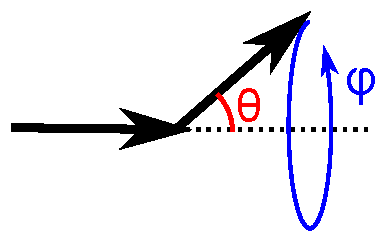
\includegraphics[width=0.5\textwidth]{\figpath/Model2_freelyrotating}}
			\end{minipage}\begin{minipage}[c]{0.45\textwidth}
				\begin{equation*}
					\langle h^2\rangle = n l^2 \left[\frac{1+\cos\theta}{1-\cos\theta}\right]
				\end{equation*}
			\end{minipage}
		
		\item The \emph{hindered-rotation} chain.  In this model, the bond angle $\theta$ is fixed, and some rotation angles $\phi$ are more favorable than others (e.g. because of sterics within the molecule):
		
			\begin{minipage}[c]{0.45\textwidth}
				\centerline{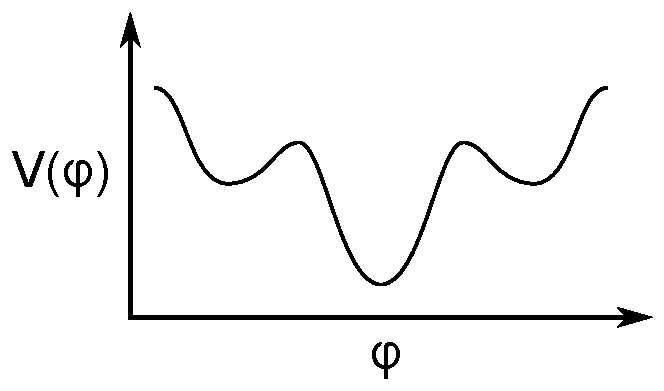
\includegraphics[width=0.5\textwidth]{\figpath/Model2_hindered}}
			\end{minipage}\begin{minipage}[c]{0.45\textwidth}
				\begin{equation*}
					\langle h^2\rangle = n l^2 \left[\frac{1+\cos\theta}{1-\cos\theta}\right] \left[\frac{1+\langle \cos\phi\rangle}{1-\langle\cos\phi\rangle}\right]
				\end{equation*}
			\end{minipage}
			
	\end{enumerate}
	
\end{model}

\begin{ctqs}

	\question As you may notice, for each of these models, $\langle h^2\rangle$ can be written in the form \label{\labelbase:ctq:C}
		\begin{equation*}
			\langle h^2 \rangle = C_\infty n l^2
		\end{equation*}
		
		Write an expression for the characteristic ratio, $C_\infty$, for...
		
		\begin{enumerate}
			\item ... the freely-jointed chain:
	
		\begin{solution}[0.5in]
			\begin{equation*}
				C_\infty = 1
			\end{equation*}
		\end{solution}
			
			\item ... the freely-rotating chain:
	
		\begin{solution}[0.75in]
			\begin{equation*}
				C_\infty = \left[\frac{1+\cos\theta}{1-\cos\theta}\right]
			\end{equation*}
		\end{solution}
			
			\item ... the hindered-rotation chain:
	
		\begin{solution}[0.75in]
			\begin{equation*}
				C_\infty = \left[\frac{1+\cos\theta}{1-\cos\theta}\right] \left[\frac{1+\langle \cos\phi\rangle}{1-\langle\cos\phi\rangle}\right]
			\end{equation*}
		\end{solution}
		\end{enumerate}

	\question For a chain with $n$ links of length $l$, which of these models do you expect to produce the most extended chain conformation?  Explain your group's reasoning in 2-3 complete sentences. \label{\labelbase:ctq:stiffness}
	
		\begin{solution}[1.5in]
			Qualitatively, the hindered rotation chain should produce the most extended conformation because the restrictions on the bond angles and rotation angles make it harder for the chain to ``fold back'' on itself.
			
			Quantitatively, for real polymers, $\cos\theta > 1$ and $\langle \cos\phi \rangle > 1$, so both the $\cos \theta$ and $\cos \phi$ terms in $C_\infty$ for the hindered rotation chain are greater than 1 and increase the mean-square end-to-end distance of the chain relative to both of the other chain models.
		\end{solution}

	
	\question The equations given in Model \ref{\labelbase:mdl:chainmodels} express the chain dimensions in terms of the number of bonds $n$ and the bond length $l$.  However, it is often also useful to describe a polymer in terms of the ``closest equivalent'' freely-jointed chain. \label{\labelbase:ctq:statseg}
	
		\begin{enumerate}
			\item  If the ``closest equivalent'' freely-jointed chain has $N$ links of length $b$, how long would the chain be if it were fully extended? \label{\labelbase:ctq:Nb}
	
		\begin{solution}[0.75in]
			\begin{equation*}
				h_{max} = Nb
			\end{equation*}
		\end{solution}
			
			\item What would the mean-square end-to-end distance of the chain be? \label{\labelbase:ctq:Nb2}
	
		\begin{solution}[0.75in]
			\begin{equation*}
				\langle h^2 \rangle = Nb^2
			\end{equation*}
		\end{solution}
		
		\end{enumerate}
		
	\question The link length $b$ is called the \emph{Kuhn length}.  Do you expect the Kuhn length to have a simple physical interpretation?  Briefly explain your group's reasoning in 2-3 complete sentences.\label{\labelbase:exc:statseginterp}
	
		\begin{solution}[1.25in]\instructordisplay{
			No, the Kuhn length does not have a simple physical interpretation.  The $N$ in this expression is \emph{not} the real degree of polymerization of the chains (see Exercise \ref{\labelbase:exc:statseg}), and $b$ is \emph{not} the actual physical size of the monomers.  They are simply proxies for the properties of the ``closest equivalent'' freely-jointed chain.
			}\studentdisplay{}
		\end{solution}
	
	\question Finally, in many experiments, it is easier to measure the \emph{radius of gyration} for a polymer chain (the mean square distance between the monomers and the polymer's center of mass), $R_g$.  For the ideal chains described in Model \ref{\labelbase:mdl:chainmodels}, it can be shown that
		\begin{equation*}
			\langle R_g^2\rangle = \frac{\langle h^2\rangle}{6}
		\end{equation*}
		
		\begin{enumerate}
			\item Find an expression for $\langle R_g^2 \rangle$ in terms of $N$ and $b$.
	
		\begin{solution}[0.75in]
			\begin{equation*}
				\langle R_g^2 \rangle = \frac{Nb^2}{6}
			\end{equation*}
		\end{solution}
			
			\item If you were to double the length of the chain, by what factor would you expect the radius of gyration to increase?
	
		\begin{solution}[0.75in]
			Replacing $N$ with $2N$ would increase $\langle R_g^2 \rangle$ by a factor of 2. Taking the square root, we find that $R_g$ would increase by a factor of $\sqrt{2}$.
		\end{solution}
			
			\item Explain, in 1-2 complete sentences, why we might say that the radius of gyration ``scales as'' the square root of the chain length.
	
		\begin{solution}[1.5in]
			$\langle R_g^2 \rangle$ is directly proportional to the degree of polymerization, which means that $\langle R_g^2 \rangle$ is directly proportional to both the extended length of the chain and the molecular weight of the chain.  Taking the square root, we find that the root mean square radius of gyration is directly proportional to the $\sqrt{N}$.  Thus the radius of gyration is proportional to (or scales as) the square root of the chain length/molecular weight.
		\end{solution}
		\end{enumerate}
	
\end{ctqs}

%\begin{model}[Radius of Gyration]
%	\label{\labelbase:mdl:Rg}
%	...
%\end{model}
	
	
\begin{exercises}
	\exercise Of the chain models shown in Models \ref{\labelbase:mdl:chainmodels}, which one would you expect to be most appropriate for describing the conformations of a polyethylene chain?  Briefly defend your reasoning in 2-3 complete sentences.  Then, substitute in appropriate values of $n$, $l$, and (if appropriate) $\theta$ and $\phi$ to estimate the radius of gyration for a polyethylene chain with a molecular weight of 700~kg/mol.
	
		\begin{solution}\instructordisplay{
			The hindered rotation model should be most appropriate for describing a polyethylene chain.  First, we know that the bond angles in polyethylene cannot have any value - they must be close to 109 degrees since the carbon centers have tetrahedral geometry.  Thus the freely-jointed chain is not a reasonable approximation.  Second, the dihedral angle $\phi$ is probably not going to be able to rotate freely, because we know that the sterics make gauche conformations of the chain less favorable than trans conformations.    This means that the hindered rotation model should be more appropriate than the freely rotating chain model.
			
			We can estimate the parameters needed to apply this model as follows:
			\begin{itemize}
				\item For the 700~kg/mol polymer described in the problem, the degree of polymerization is $N = (700\text{ kg/mol})/(28\text{ g/mol}) = 25000$.  
				\item Because each monomer contributes 2 C-C bonds to the polymer backbone, $n=2N=50000$ (remember that $n$ counts bonds, not monomers!).  
				\item A typical C-C bond has length $l=1.5\AA$. 
				\item The bond angle is approximately $109^\circ$ - but note that $\theta$ is defined as the supplement of what we conventionally think of as the bond angle, so we should use $\theta=180-109^\circ = 71^\circ$.  
				\item $\langle \cos \phi\rangle$ is tricky, since $\phi$ can take any value but will have some more probable than others. For simplicity, we'll do the calculation with $\phi=90^\circ = \pi/2$, but this isn't really physically accurate.
			\end{itemize}
			
			Using these numbers to calculate $C_\infty$, we find
			\begin{align*}
				C_\infty &= \left[\frac{1+0.33}{1-0.33}\right]\left[\frac{1+0}{1-0}\right]\\
				&= 1.98
			\end{align*}
			(The literature value for $C_\infty$ for polyethylene is 7.4, which suggests that we should have used a value of $\langle\cos\phi\rangle$ closer to 0.6, but our rough estimate gets us into the right ballpark.)
			
			Finally,
			\begin{align*}
				\langle R_g^2\rangle &= \frac{\langle h^2\rangle}{6}\\
				&= \frac{C_\infty n l^2}{6} \\
				&= 1.98(50000)(1.5\,\AA)^2/6\\
				&= 37500\,\AA^2
			\end{align*}
			so $R_g \approx \sqrt{37500\,\AA^2} = 190\,\AA = 19\text{ nm}$.
		}\end{solution}

	\exercise A useful rule of thumb for estimating radius of gyration is that the radius of gyration for polymers with a molecular weight of $10^5$ g/mol is typically about 10~nm.
	
		\begin{enumerate}
			\item Using what you learned about how radius of gyration scales with the length of a polymer chain (and thus its molecular weight), predict the radius of gyration of a polymer with a molecular weight of $2\times10^5$~g/mol.
	
		\begin{solution}\instructordisplay{
			The easiest way to solve this problem is to set up a ratio:
				\begin{equation*}
					\frac{R_{g,1}^2}{R_{g,2}^2} = \frac{N_1}{N_2} = \frac{M_1}{M_2}
				\end{equation*}
				(where we can switch from degree of polymerization, $N$, to molecular weight, $M$, because they are directly proportional to each other and the proportionality constant ($M_0$) cancels out when we take the ratio).
				
			Thus
			\begin{align*}
				R_{g,1} &= \sqrt{ R_{g,2}^2 \frac{M_1}{M_2} }\\
					&= R_{g,2} \sqrt{\frac{M_1}{M_2}}\\
					&= (10\text{ nm})\sqrt{\frac{2\times 10^5\text{ g/mol}}{10^5\text{ g/mol}}}\\
					&= 14\text{ nm}
			\end{align*}
		}\end{solution}
			
			\item Using a similar approach, predict the molecular weight of a polymer with a radius of gyration of 100~nm.
	
		\begin{solution}\instructordisplay{
			This solution is similar to above.  Rearranging to solve for $M_2$:
			\begin{align*}
				M_2 &= M_1\frac{R_{g,1}^2}{R_{g,2}^2}\\
				&= (10^5\text{ g/mol})\frac{(100\text{ nm})^2}{(10\text{ nm})^2}\\
				&= 10^7\text{ g/mol}
			\end{align*}
		}\end{solution}
		\end{enumerate}
		
	\exercise \label{\labelbase:exc:statseg} The relationship between a polymer chain and its ``closest equivalent'' freely-jointed chain can be a bit confusing.  Explore this idea in more detail by doing the following:
	
		\begin{enumerate}
			\item Combine your answers to CTQs \ref{\labelbase:ctq:statseg}a and b with the expression for $\langle h^2\rangle$ given in CTQ \ref{\labelbase:ctq:C}, and solve for $N$ and $b$ in terms of $C_\infty$, $n$, $l$, and the maximum end-to-end distance of the polymer chain, $h_{max}$.
				
				\begin{solution}\instructordisplay{
					In CTQ \ref{\labelbase:ctq:statseg}b, we wrote
					\begin{equation*}
						\langle h^2 \rangle = Nb^2
					\end{equation*}
					Combining this with the expression from CTQ \ref{\labelbase:ctq:C}, we obtain
					\begin{equation*}
						C_\infty n l^2 = Nb^2
					\end{equation*}
					From CTQ \ref{\labelbase:ctq:statseg}a, we also know that $h_{max} = Nb$, so
					\begin{align*}
						C_\infty n l^2 &= h_{max} b\\
						b & = \frac{C_\infty n l^2}{h_{max}}
					\end{align*}
					Finally, we can solve for $N$ using
					\begin{align*}
						N &= \frac{h_{max}}{b}\\
						&= \frac{h_{max}^2}{C_\infty n l^2}
					\end{align*}
				}\end{solution}
			
			\item Consider a polystyrene chain with $M_n=10\text{ kg/mol}$.
			
				\begin{enumerate}
					\item What is the number-average degree of polymerization of this chain?
				
				\begin{solution}\instructordisplay{
					For polystyrene, $M_0=104\text{ g/mol}$ so
					\begin{equation*}
						N = \frac{10\text{ kg/mol}}{104\text{ g/mol}} = 96
					\end{equation*}
				}\end{solution}
				
					\item What should the maximum end-to-end distance for this chain be?  (Hint: use what you learned in Model \label{size-and-complexity:mdl:polyethylenesize} in Activity 1.\ref{size-and-complexity}!)
				
				\begin{solution}\instructordisplay{
					As we learned in Activity 1.\ref{size-and-complexity}, every 2 C-C bonds in the polymer backbone contribute approximately 0.25~nm to the contour length of the polymer. Thus,
					\begin{align*}
						h_{max} &= (96\text{ monomers})\left(\frac{2\text{ C-C bonds}}{\text{monomer}}\right)\left(\frac{0.25\text{ nm}}{2\text{ C-C bonds}}\right)\\
						&= 24\text{ nm}
					\end{align*}
				}\end{solution}
					
					\item For polystyrene, $C_\infty=9.5$, and each C-C bond in the backbone has length $l\approx 1.5\,\AA$.  Using this information, calculate $N$ and $b$ for the equivalent freely-jointed chain. (Hint: remember that $n$ counts bonds, not monomers!)
				
				\begin{solution}\instructordisplay{
					Since there are 96 monomers in the chain, there are $n=192$ C-C bonds.  Plugging these numbers into the expression from part (a), we obtain
					\begin{align*}
						N &= \frac{(240\,\AA)^2}{9.5\cdot 192\cdot(1.5\,\AA)^2}\\
							&= 14\\
						b &= \frac{9.5\cdot 192 \cdot (1.5\,\AA)^2}{240\,\AA}\\
						&= 17.1\,\AA
					\end{align*}
				}\end{solution}
				
				\item Compare your answers to parts (a) and (c), and use your results to critique or defend the following statement:
				
					\emph{``The number of links in the closest equivalent freely-jointed chain is equal to the actual degree of polymerization of the polymer, and the Kuhn length corresponds to the effective size of a single chemical repeat unit.''}
				
				\begin{solution}\instructordisplay{
					Based on the numbers calculated in this question, this statement is clearly false.  The actual degree of polymerization is 96, while the number of Kuhn segments is only 14.  Similarly, the Kuhn length is 17~\AA (1.7~nm), but this is much too large to correspond to a single styrene repeat unit.  Thus, as discussed in CTQ \ref{\labelbase:exc:statseginterp}, the Kuhn length (and number of Kuhn segments in the closest equivalent freely-jointed chain) DO NOT have a simple physical interpretation in terms of the number and size of the chemical repeat units in the chain.
				}\end{solution}
				
				\end{enumerate}
		\end{enumerate}
		
\end{exercises}
	
\end{activity}